\chapter{Perspectives}

In this thesis, I introduced the \HubLem fragmentation model and applied it to the dynamical evolution of substructured star clusters, also exploring the fate of their binary population. Interesting results have been obtained, though some assumptions were made. In this chapter, I review two of these assumptions:  the isolated nature of the cluster and the absence of stellar evolution.  I also present a method to obtain elongated fragmented models, and describe the outline of a comparison to observations. Finally I discuss the inclusion of hydrodynamical effects in the model.


\minitoc



\section{Tidal field}

In all our simulations, it was assumed the clusters were in isolation and no tidal field was applied. This allowed us to study the mechanisms of violent relaxation and the erasure of substructure. However, in reality, star forming regions are shaped by the gravitational influence of their surroundings. We mentioned in section \ref{Sec:2_conclusion} that the galactic tidal field could prevent the collapse of the \HubLem fragmented configuration and scatter the clumps, injecting them in the galactic cluster mass function. The fate of these clumps is uncertain, as some will disperse through two-body interactions, and other will merge, depending on the geometry imposed by the tidal field. 


The tidal shear caused by differential rotation is important on large enough scales. \cite{BT} give the Jacobi radius of a cluster on a circular orbit at the solar galactocentric radius:
\begin{equation}
r_j = \left( \frac{G m}{4 \Omega_0 A_0} \right)^\frac{1}{3} = 52~\pc \left( \frac{m}{10^5~\Mo} \frac{\Omega_0}{A_0} \right)^\frac{1}{3} \left( \frac{220 \textrm{km.s}^{-1}}{v_c} \frac{R_0}{8~\textrm{kpc}} \right)^\frac{2}{3},
\end{equation}
with $m$ the cluster mass, $\Omega_0$ the angular galactic rotation, $A_0$ an Oort constant and $v_c$ the tangential velocity at the galactocentric radius $R_0$. Substructures spanning more than 50 pc in a regular galactic environment are expected to be strongly affected by tidal shear, modifying the merging rate.

Numerical simulations will enable an exploration of the resulting clump mass function, which would be more directly comparable to the cluster mass function in the Galaxy. NBODY6 has a built-in galactic tidal field module, which allows the user to model the tidal forces associated with the cluster orbiting a complex galactic potential, including a \cite{Miyamoto1975} potential, see \cite{Aarseth2003} for details. The tidal shock from a passing molecular cloud is also an option in NBODY6.

It is possible to go further in the inclusion of realistic tidal fields. \cite{Renaud2011} introduced a new version of NBODY6, \href{http://personal.ph.surrey.ac.uk/~fr0005/nbody6tt.php}{Nbody6tt}, that can take an arbitrary tidal tensor as an input and apply it to the evolution of a star cluster. Specifically, Nbody6tt enables the application to a cluster of a tidal environment extracted from a large-scale galactic simulation to obtain a time-dependant, self-consistent tidal field. The influence of different galactic environment, such as tidal arms, on the cluster can then be evaluated. 

For example, \cite{Renaud2015b} reported the formation of massive clusters in their hydrodynamical simulation of a galaxy merger analog to the Antennae galaxies. Fig~\ref{Fig:7_renaud} show the merging of YMC fragments on 100~pc scales. This kind of event could be reproduced in Nbody6tt with a \HubLem configuration and the tidal data from the simulation. Given the complex tidal fields in this kind of environment, the evolution of YMCs starting from substructured initial conditions could shed light of their formation and disruption processes, among which the tidal shear mentioned earlier.


\begin{figure}
\begin{center}
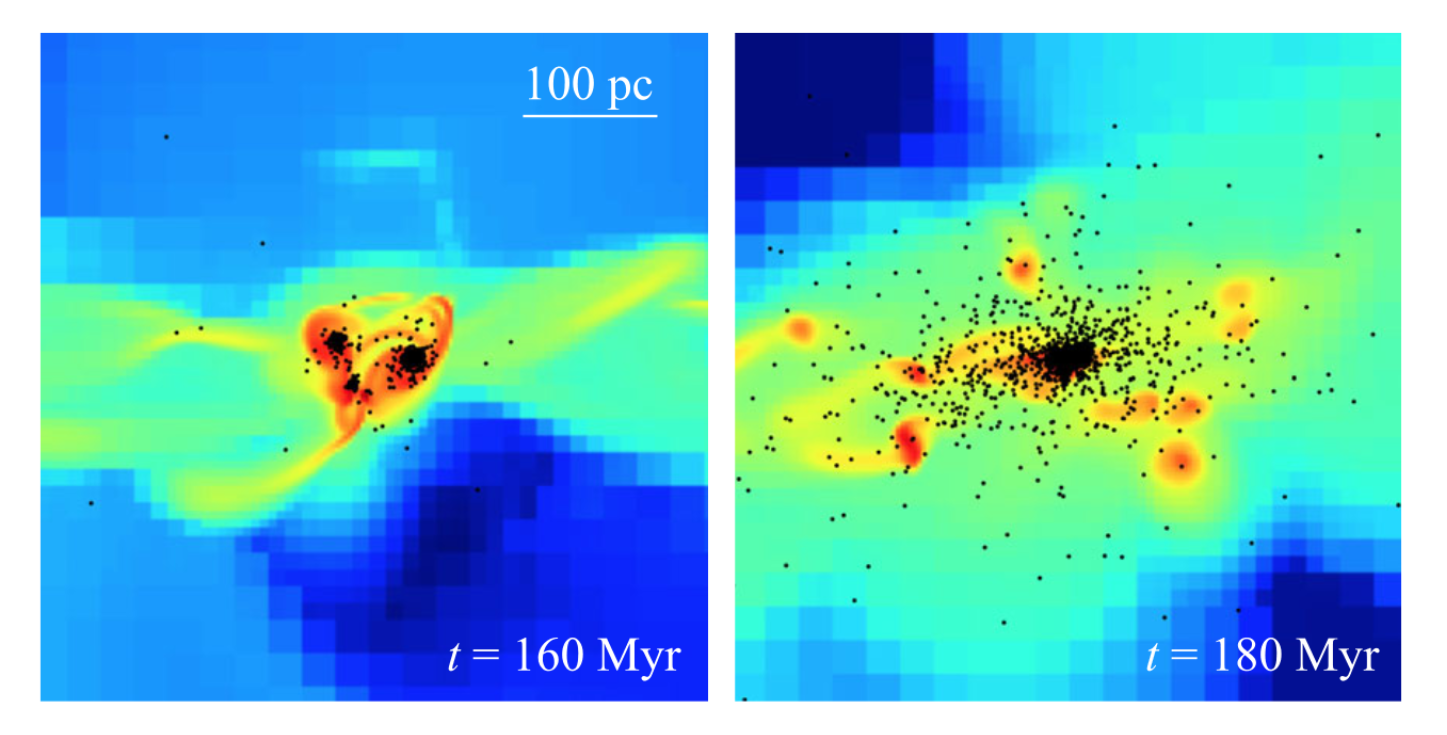
\includegraphics[width=0.7\textwidth]{Figures/7_renaudantennas.png}
\end{center}
\caption[Cluster formation in a hydrodynamical simulation of the Antennae galaxies]{Cluster formation in a hydrodynamical simulation of the Antennaes galaxies. The colormap indicates gas densities and newly formed stars are shown as black dots. Two epochs are shown, outlining the erasure of substructure. The figure was extracted from \cite{Renaud2015b} }
\label{Fig:7_renaud}
\end{figure} 



\section{Stellar evolution}





No stellar evolution effects were included in our simulations. While choosing our maximum stellar masses (tables \ref{Tab:2_models} and \ref{Tab:6_models}) and the physical duration of our simulations (sections \ref{Sec:3_Scaling} and \ref{Sec:6_models}), we assumed stellar evolution would not significantly impact the global dynamical evolution of the substructured fragmented configurations. However, these mass ranges do not reflect the extent of the stellar mass spectrum observed in some young clusters; an often cited upper limit on stellar masses is 150~$\Mo$ \citep{Oey2005}.

As we shown in chapter~\ref{Chap:nbody}, these stars would seed the fragmentation of the cluster and shape the clump mass function. Would their subsequent evolution affect the internal dynamics of clumps in our models ? To answer this, we turn to stellar models. Fig~\ref{Fig:7_stellarlifetime_hurley} shows the time needed for a star to reach the Giant Branch, the main-sequence lifetime, as a function of its mass. This analytical model from \cite{Hurley2000} reaches up to $\sim$ 60~$\Mo$, which gives a main-sequence lifetime of 6 Myr, while in our least dense models, with an initial stellar density of 6 stars/$\pc^{-3}$, the clumps take 6 Myr to merge and erase the substructure.

However, if we include the tidal fields from last section, the clumps might survive far longer, and the death of these massive stars could have a significant impact on their structures, their mass segregation, and  on the overall clump mass function.

Moreover, more massive stars than 60 $\Mo$ are observed in clusters, and the lifetime alone does not reflect the mass-loss these stars endure throughout their life. Fig~\ref{Fig:7_stellarlifetime_weidner} shows the evolution of mass for several massive stars, 50, 65, 85 and 120~$\Mo$, from the Geneva stellar model \citep{Schaller1992}. These stars not only disappear in less than 4 to 5 Myr, they also lose a non-negligible portion of their mass before their death.

Throughout this thesis, we assumed stellar evolution would not affect the dynamics of our simulated clusters. For isolated systems, and for the densities and mass ranges we chose, this is mostly true. Nevertheless, as we include tidal fields and an extended mass spectrum to reproduce observed objects, mass-loss and other evolutionary effects need to be taken into account. This is especially true for binary evolution. Mass loss would affect the binary parameters, and some binaries found in our systems have short enough separations to be contact binaries, had stellar radii and evolution be included. These objects may be important for the formation of blue stragglers or black holes, as they speed up stellar evolution.

NBODY6 has a built-in stellar evolution module based on the analytical model by \cite{Hurley2000}, including wind-driven mass loss, radii evolution, supernova event and stellar remnants. It was not used in this work for simplicity, but should be used for further research.



\begin{figure}
    \centering
    \begin{subfigure}[b]{0.60\textwidth}
        \centering
        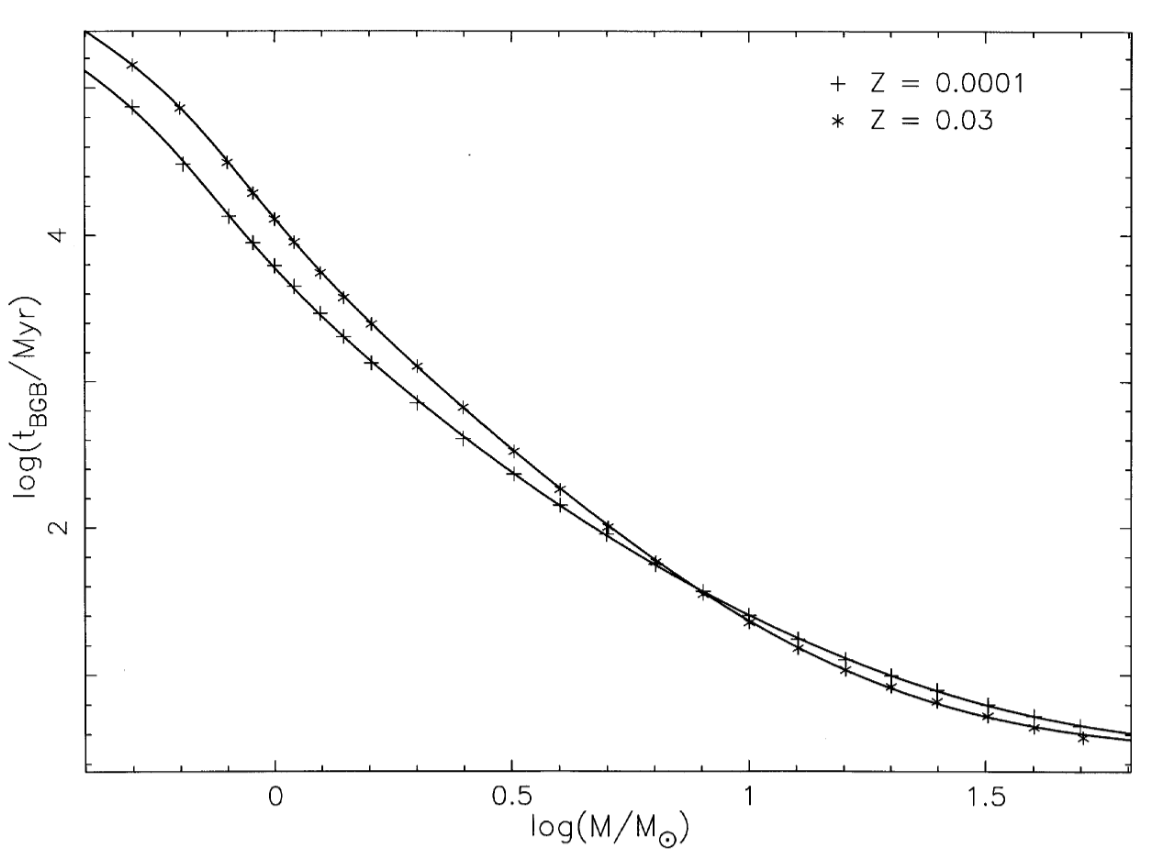
\includegraphics[width=0.85\textwidth]{Figures/7_stellarlifetime.png}
        \caption{Time to reach the giant branch vs stellar mass.}
        \label{Fig:7_stellarlifetime_hurley}
    \end{subfigure}
    \begin{subfigure}[b]{0.38\textwidth}
        \centering
        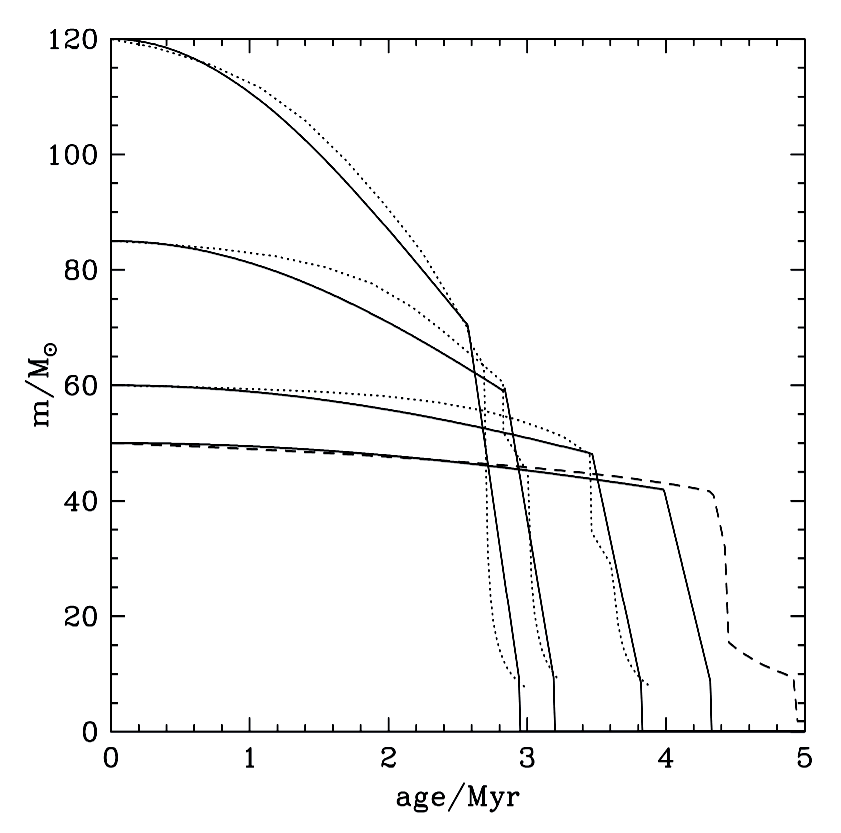
\includegraphics[width=\textwidth]{Figures/7_stellarlifetime_weidner.png}
        \caption{Mass loss for massive stars.}
        \label{Fig:7_stellarlifetime_weidner}
    \end{subfigure}
     \caption[Stellar evolution models]{(a) Time taken to reach the Base of the Giant Branch (BGB) as a function of initial stellar mass, for two metallicities, Z = 0.0001 and Z = 0.03. The figure was extracted from \cite{Hurley2000}. (b) Evolution of mass over time for several massive stars, based on the Geneva stellar model \citep{Schaller1992}. The figure was extracted from \cite{Weidner2006}. }
     \label{Fig:7_stellarlifetime}
\end{figure}




\section{Anisotropic expansion}

The \HubLem expansion we used throughout this thesis was isotropic, the velocity field was expressed with $\bold{v} = \Hub_0 \bold{r}$ with \tHub a scalar value. As a result, the fragmented configurations are roughly spherical and the net systemic angular momentum is null. This is a key difference between the method we have developed and the fractal approach of \cite{Goodwin2004}. Angular momentum may be significant in young clusters such as R136 \citep{Henault-Brunet2012}. In a fractal model, the way the velocity field is built leaves a residual, global angular momentum whereas the \HubLem approach starts off with strictly zero angular momentum.

 A net angular momentum could be introduced in a Hubble model, for instance by setting 
\begin{equation}
\bold{v} = \Hub_o \bold{r} + \bold{\Omega} \times \bold{r}
\end{equation} 
with $\bold{\Omega}$ a chosen angular velocity. One can actually go further and write in matrix form
\begin{equation}
\bold{v} = \hat{\bold{H}} \bold{r} = \left(\begin{matrix}
H_{x,x} & H_{x,y} & H_{x,z}\\
H_{y,x} & H_{y,y} & H_{y,z}\\
H_{z,x} & H_{z,y} & H_{z,z}\\
\end{matrix}\right) \bold{r},
\end{equation}
with $\hat{\bold{H}}$ now a 3$\times$3 matrix, where the off-diagonal elements account for rotation and the elements on the diagonal $\Hub_{ii}$ control the three dimensional expansion. In this study, we have set $\Hub_{ij,i\ne j}=0$ and $\Hub_{ii}=\Hub_o$ otherwise. It is then a simple matter to study the fragmentation along a filament by setting, for example, $\Hub_{xx}=\Hub_{yy} < \Hub_{zz}$. 


\begin{figure}
    \centering
    \begin{subfigure}[b]{\textwidth}
        \centering
        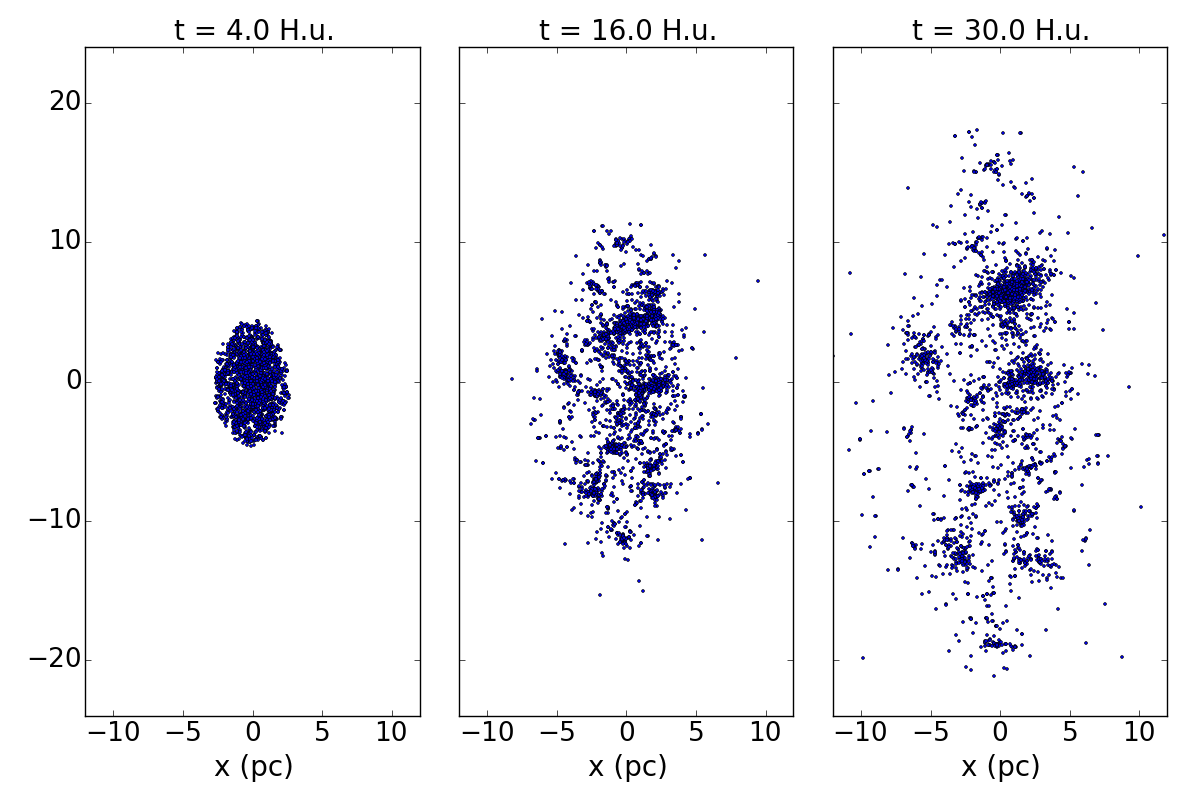
\includegraphics[width=0.85\textwidth]{Figures/7_anisotropic.png}
        \caption{Anisotropic \HubLem expansion.}
        \label{Fig:7_anisotropic}
    \end{subfigure}
    
    \begin{subfigure}[b]{0.6\textwidth}
        \centering
        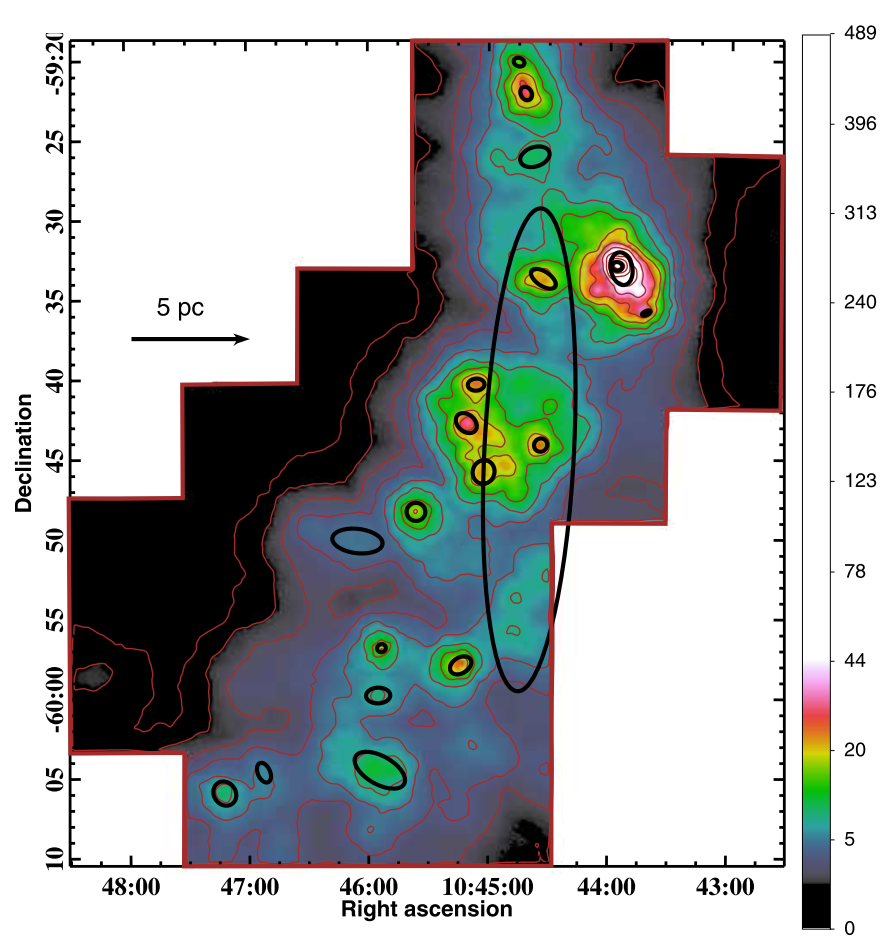
\includegraphics[width=\textwidth]{Figures/7_carina.png}
        \caption{Stellar density in Carina.}
        \label{Fig:7_carina}
    \end{subfigure}
     \caption[Example of anisotropic expansion and comparison to Carina]{(a) Evolution of an anisotropic \HubLem model. The expansion was favoured along z and a rotation around the same axis was introduced. (b) Stellar density in the young Carina cluster; the colorbar is in stars/$\pc^3$. The figure was extracted from \protect\cite{Kuhn2014}.}
     \label{Fig:7_filament}
\end{figure}




For example, to favor fragmentation along the z-axis and introduce a rotation along the same axis, the matrix can take the form
\begin{equation}
\bold{v} = \left(\begin{matrix}
0.2 + \cos \theta &  -\sin \theta & 0\\
\sin \theta & 0.2 + \cos \theta & 0 \\
0  & 0 & 1.7\\
\end{matrix}\right) \bold{r},
\end{equation}

with $\theta$ setting the orientation and strength of the rotation. We set $\theta = \frac{\pi}{4}$ and show the evolution of the resulting system with N=3000 on Fig~\ref{Fig:7_anisotropic}. We obtain an elongated substructured configuration, that is comparable to the observed structure of, e.g., the Carina star forming region as observed in the MYStIX survey \citep{Kuhn2014} shown on Fig~\ref{Fig:7_carina}.



\section{Mock observations}

Another path of research with the \HubLem models is the generation of mock observations to investigate completeness effects on the observed morphology of young clusters. In this section we demonstrate a proof of concept of the method.

\subsection*{Observed mass segregation in low-density star-forming regions}

We mentioned in the introduction that \cite{Bressert2010} argue for a star formation proceeding from a continuous spatial distribution, instead of distinct "isolated" and "clustered" formation modes. The authors found a stellar surface density distribution for YSOs to be log-normal, peaked around 22 stars/$\pc^{-2}$.  High density young clusters would be the result of the dynamical evolution we described in this thesis, with local low-density clumps and overdensities merging and populating the high density tail of the observed distribution.

While there seems not to be a clear distinction between isolated and clustered star-formation, the dynamical processes at play are expected to be different, as low density imply a low crossing times. Thus stars forming in low density clumps should not be expected to undergo significant dynamical evolution, and their characteristics should impact the outcome of their mergers.

\cite{Kirk2011} adressed this issue by investigating the distribution of Young Stellar Objects in low-density star forming regions, especially their degree of mass segregation. Their target objects, among which IC 348 and Chal I, are substructured and show multiple stellar clumps. To measure mass-segregation in such spatial distributions, they used the Minimum Spanning Tree method to isolate clumps and evaluate their individual mass segregation.

They found some mass segregation, often limited to to the most massive star. However, it is important to note that such structure analysis is very  sensitive to completeness. The most massive stars are the most luminous and in case of mass segregation, sit in the center of clumps. Including lighter, fainter and more spread out stars could alter the global spatial distribution, change the spanning tree and potentially connect clumps, modifying the mass segregation measures. This problem could be worsen by the fact that the dust in the galaxy is substructured, which could also influence the observed objects close to the detection limit.

Their objects are close enough ($\sim$200~pc) for this not to be a significant problem, but it could be for more distant objects. We wish to  demonstrate how to use our naturally mass-segregated and substructured model to generate mock observations and assess the influence of completeness on the structure analysis of these objects. To do so, we will reproduce a model similar to IC 348, attribute luminosities to the stars and take dust extinction into account.


\subsection*{Making our own IC 348 and turning on our stars}


We focus on IC 348 and reproduce a similar cluster. We first perform a \HubLem expansion with N=400, the estimated membership of IC 348. As seen on Fig~\ref{Fig:7_MSTedge}, The structure is quite irregular compared to most of the roughly spherical models we shown in this thesis, this is due to a stronger fragmentation caused by the low number of stars.

To attribute luminosities to these stars, we use the stellar evolution code \href{http://mesa.sourceforge.net/}{MESA} \citep{Paxton2011}, a detailed suite of simulation tools able to model a star from protostar to white dwarf. Given the young age of IC 348, we are mainly interested in the pre-main-sequence and early main-sequence luminosities. We fix the age to 3 Myr, as the results appear weakly affected by age dispersion. The code ouputs bolometric luminosities, that we can convert to apparent bolometric magnitude $m_{bol}$ through

\begin{equation}
m_{bol} = 4.74- 2.5 \log\left(\frac{L_{bol}}{L_\odot}\right) - 2.5\log\left( \frac{d}{10~\pc}\right).
\end{equation}




We convert these bolometric magnitude to H band magnitudes with a script, \textit{Starflux}. Starflux takes the bolometric luminosity from the tables of \cite{Hurley2000} and computes bolometric corrections based on the \href{http://www2.iap.fr/pegase/pegasehr/#codes}{PEGASE stellar library}.


 We consider two different distances of 300 pc (the current estimate for IC 348) and 1 kpc to evaluate the effects of distance with a fixed detection limit.

\subsection*{Dust extinction}

Finally, we take dust extinction into account with the work of \cite{Green2015}. The authors gathered PAN-STARRS 1 and 2MASS data to obtain a 3D dust extinction map in the Galaxy covering 75\% of the sky. The database is downloadable through their \href{http://argonaut.skymaps.info/}{website}, which also accepts custom queries to obtain the color excess $E_{B-V}$ for any user-requested coordinates and distance.

\cite{Niederkorn2016} built a software to obtain extinction map from the user input of coordinate range, distance and spatial resolution. The software automatically handles the query process to get each extinction pixel. It also converts the color excess $E_{B-V}$ to the H-band extinction $A_H$ through the relation
\begin{equation}
A_H =   \frac{E_{B-V}}{ \frac{A_B/A_V}{A_H/A_V} - \frac{1}{A_H/A_V} },
\end{equation}
in which the ratios $A_B/A_V$ and $A_H/A_V$ are based on the correlations observed by \cite{Cardelli1989}. 


\begin{figure}
\begin{center}
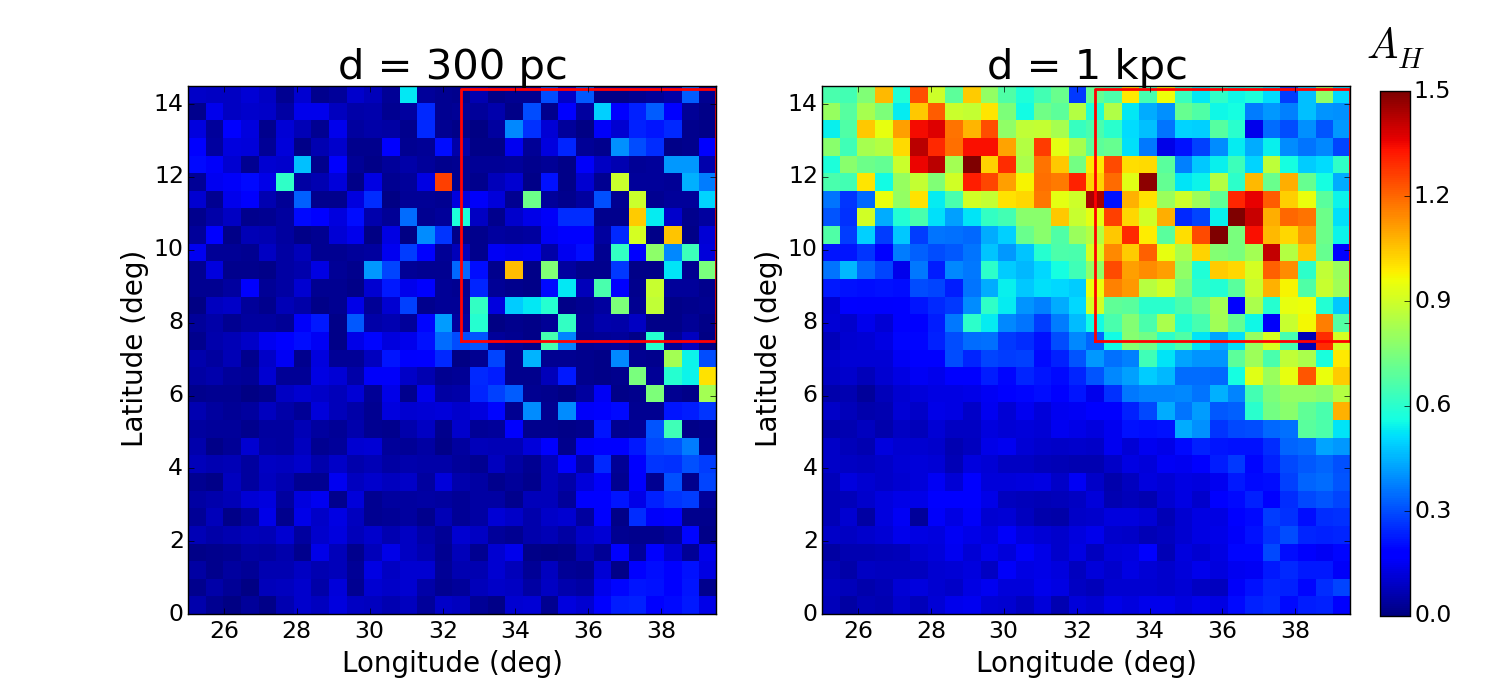
\includegraphics[width=\textwidth]{Figures/7_dustmaps.png}
\end{center}
\caption[Extinction map in H band for selected coordinates]{Extinction map in H band obtained from our script and \cite{Green2015}. Left panel shows the extinction at 300~pc and right panel at 1~kpc. The red square shows the zoomed in map we applied to our models.}
\label{Fig:7_dustmaps}
\end{figure} 

We select, at random, a region of the sky with longitude spanning from 25° to 40° and latitude from 0° to 15°, as a 30$\times$30 pixels map. We show on Fig~\ref{Fig:7_dustmaps} the two extinction maps obtained from the map of \cite{Green2015} and Niederkorn's script. They are, as mentioned earlier, heavily substructured. We are now equiped to generate mock observations of a young substructured star clusters, including dust extinction. We take our \HubLem N=400 model with the appropriate H magnitudes and apply the extinction map within the red square of Fig~\ref{Fig:7_dustmaps}, chosen to maximize the extinction for this proof of concept.

\subsection*{Observed structure}


\begin{figure}
\begin{center}
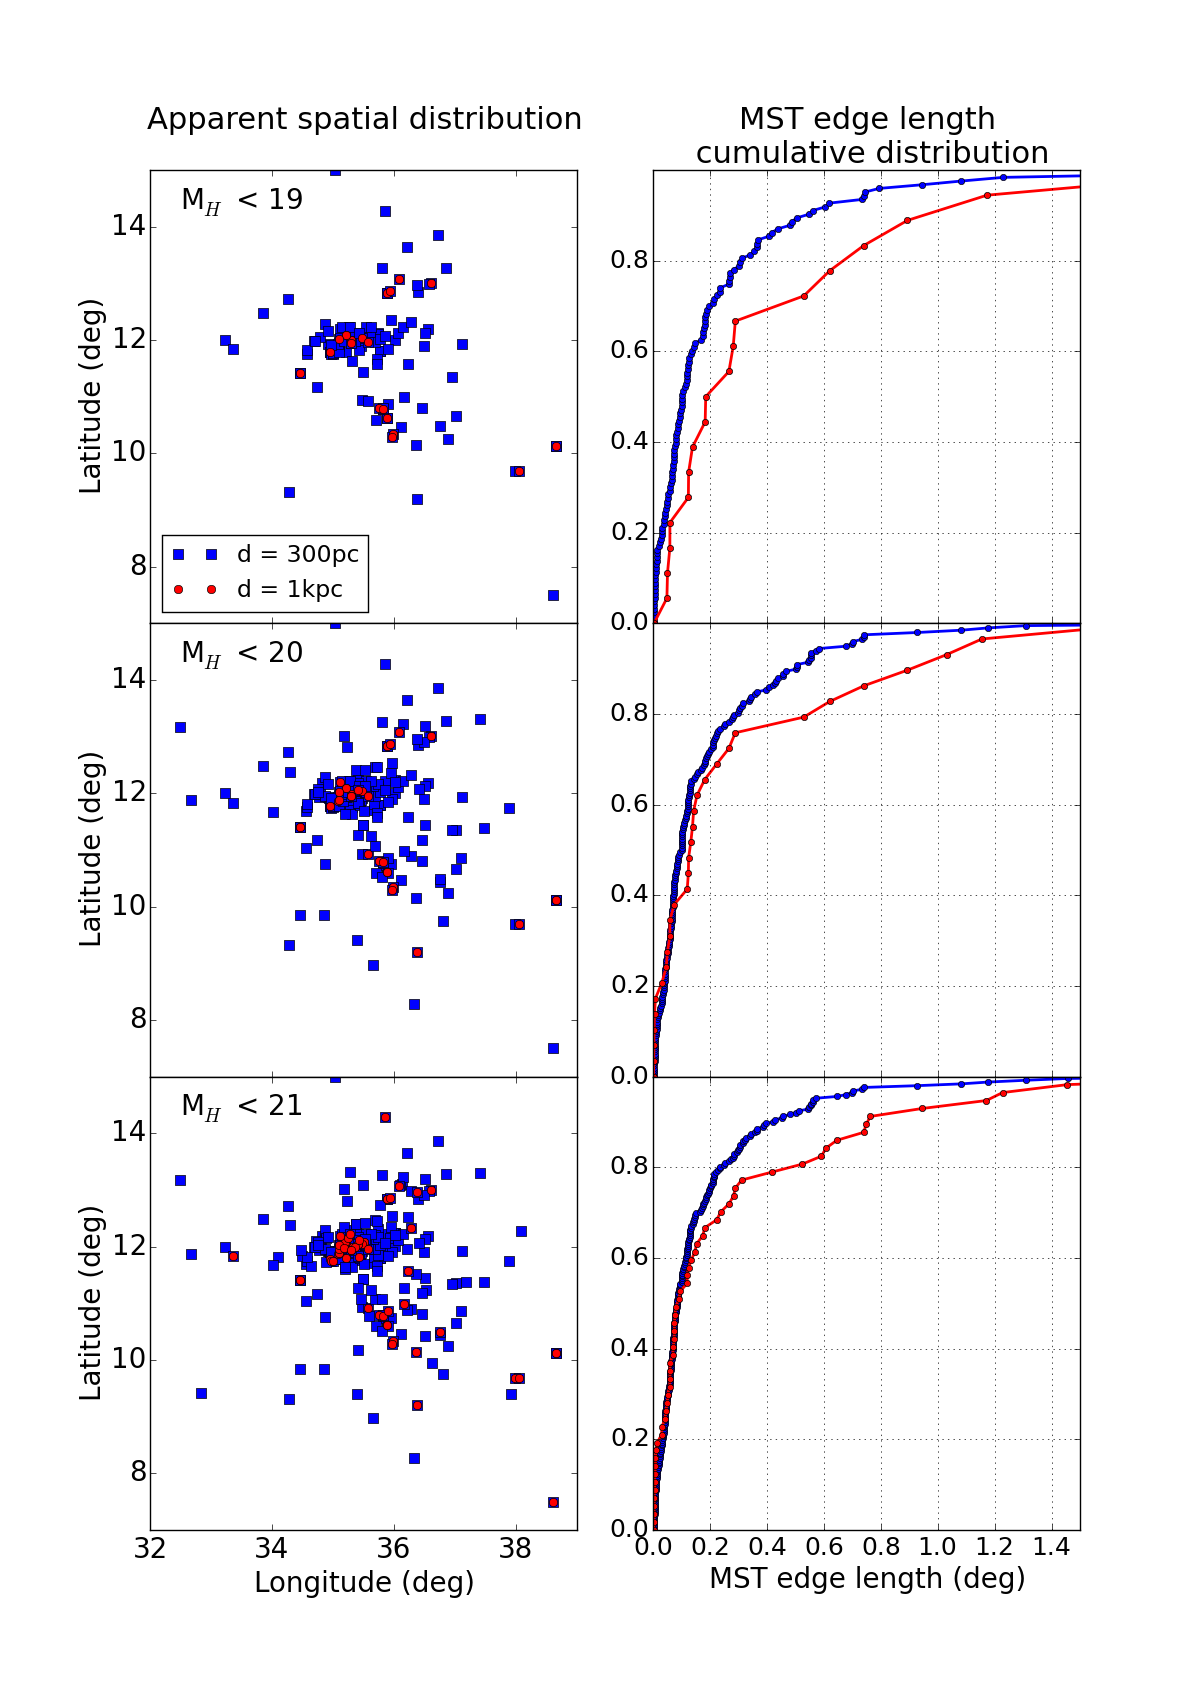
\includegraphics[width=0.98\textwidth]{Figures/7_MSTedge.png}
\end{center}
\caption[Influence of extinction on cumulative distribution of MST edges]{Left panels: spatial distribution of  stars in our ``fake" IC~348 cluster that are detected with the specified detection limit in H band. Blue stars are detected at 300pc while red stars are detected at 1kpc. Right panels: normalized cumulative distribution of the MST edge lengths, the colors match the legend on the left, the 1kpc distribution is lower and shallower.}
\label{Fig:7_MSTedge}
\end{figure} 


We show on Fig~\ref{Fig:7_MSTedge} the result for 3 detection limits in H magnitude: 18, 19, 20. These were chosen to illustrate the changes underwent by the morphology as we detect more and more stars. Left panels show the stars with a magnitude below the limit for a cluster at 300~pc (blue squares) and 1~kpc (red circles). Any star detected at 1~kpc is also detected at 300~pc. Right panels show the normalized cumulative distribution of the edge lengths in the Minimum Spanning Tree computed from the corresponding configuration (similar to Fig~\ref{Fig:2_dcutcumulated}). The x-axis stops at 1.5 to better visualize the turning point, as the distributions are normalized, they both reach 1.



As the system is mass-segregated, less luminous lighter stars are more spread out in the system. As the dust or the distance make their magnitude go over the detection limit, the cluster gets clumpier, and the cumulated edge distribution gets shallower. 

This kind of analysis could be done on wider scale, with various cluster membership, density, ages or morphologies (see anistropic expansion earlier), and would bring an interesting view of the influence of mass segregation on observed morphologies. \HubLem models are ``naturally" mass-segregated, meaning the most massive stars are not automatically at the heart of clumps. This brings a variability hard to reproduce with artificially segregated models. 



\section{Hydrodynamical effects}

For now the \HubLem expansion is a gas-less process, producing pure N-body initial conditions. Though several observations do show a lot of substructures in the stellar distribution in star forming regions, they also show  substructures in the gas from which these stars emerge. \cite{Rathborne2015} report ALMA data of the molecular cloud G0.253+0.016, which they show is on the verge of undergoing a burst of star formation. The low sound speed in the $\sim 10K$ gas implies that the proto-stars will condense from the gas and be distributed spatially in a pattern of filaments similar to what is seen in the gas. In the same vein, deep IR observations of $\rho$-Ophiucus by \cite{Andre2007} reveal pre-stellar clumps of cold gas with low inter-clump velocity dispersion, of the order of $\sim$ 1 km.s$^{-1}$, also making a case  for {\it in-situ} star formation. Strong interactions between stars would still impact on the global dynamics but only during the final stages of their formation (binarity, masses of circum-stellar discs).

Finally, the In-Sync survey of \cite{Foster2015} published APOGEE spectroscopic observations of NGC 1333, a young embedded nearby open star cluster ( $\sim$ 250 pc; total mass of gas and stars $\sim10^3 M_\odot$). The $< 3 $ Myr-old main sequence stars in NGC 1333 have a 1d velocity dispersion $\sim$ 0.8 km/s which matches the expected virial dispersion given the radial mass profile. The stars are surrounded by dense, cool gaseous cores of {\it low} (sub-virial) velocity dispersions. Inspection of the spatial distribution of both the stars and the gaseous clumps shows them to be highly substructured (see their Fig. 1). There is an obvious challenge here, discussed at length by \citeauthor{Foster2015}, to explain why gas-clumps and stars should follow such remarkably different kinematics.

The \HubLem model could be used to address the transition from embedded clusters to gas-free stellar cores. This would require the addition of  a substantial amount of gas in the system. The details of the procedure are yet to be formulated, as the inclusion of a gaseous component to the expansion is not straightforward, but this is a promising way to explore closer ties with observations of young star forming regions.